% fig_mc_elements.tex
% TR-37: Protection element coverage shares (1st trip, N=3808 cleared)
% Stacked horizontal bar showing: Z1=48.9%, 87L=46.9%, 67Q=4.2%
% Plus a second row: 2nd trip elements for permanent faults (87L=100%)
%
% Simple TikZ bar chart (horizontal, two rows)

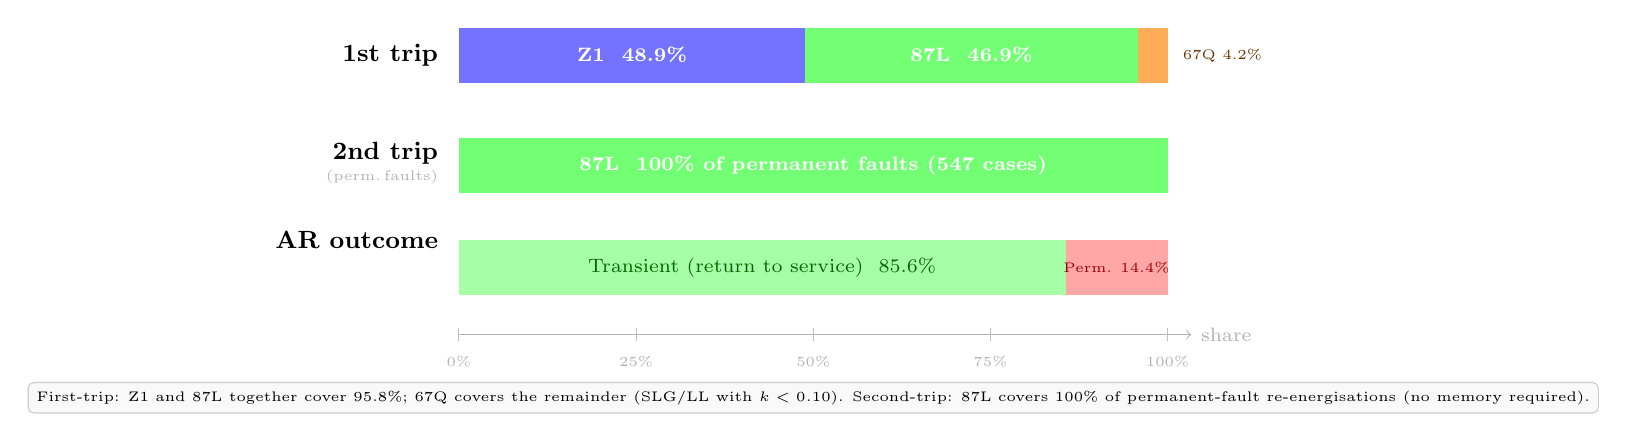
\begin{tikzpicture}[
  every node/.style={font=\scriptsize},
]

%% ── Scale: total width = 9 cm ────────────────────────────────────────────────
% Z1=48.9% → 4.40 cm, 87L=46.9% → 4.22 cm, 67Q=4.2% → 0.38 cm

\def\bh{0.70}   % bar height
\def\bw{9.00}   % total bar width

%% ── Row 1: First-trip coverage ───────────────────────────────────────────────
\node[left=4pt, font=\small\bfseries] at (0, 0.35) {1st trip};

% Z1
\fill[blue!55]    (0,      0) rectangle (4.401,  \bh);
\node[white, font=\scriptsize\bfseries] at (2.20,  0.35) {Z1 \ 48.9\%};

% 87L
\fill[green!55]   (4.401,  0) rectangle (8.622,  \bh);
\node[white, font=\scriptsize\bfseries] at (6.51,  0.35) {87L \ 46.9\%};

% 67Q
\fill[orange!65]  (8.622,  0) rectangle (9.00,   \bh);
\node[orange!40!black, font=\tiny, right=2pt] at (9.00, 0.35) {67Q 4.2\%};

%% ── Row 2: Second-trip coverage (permanent faults, 547 cases) ─────────────
\node[left=4pt, font=\small\bfseries] at (0, -0.90) {2nd trip};
\node[left=4pt, font=\tiny, gray!60] at (0, -1.20) {(perm.\,faults)};

% 87L: 100% of 547
\fill[green!55]   (0, -1.40) rectangle (9.00, -1.40+\bh);
\node[white, font=\scriptsize\bfseries] at (4.50, -1.05) {87L \ 100\% of permanent faults (547 cases)};

%% ── AR row: transient faults ──────────────────────────────────────────────
\node[left=4pt, font=\small\bfseries] at (0, -2.00) {AR outcome};

% Transient = 85.6% → 7.70 cm; Permanent = 14.4% → 1.30 cm
\fill[green!35]   (0,    -2.70) rectangle (7.704,  -2.70+\bh);
\node[green!40!black, font=\scriptsize] at (3.85, -2.35) {Transient (return to service) \ 85.6\%};

\fill[red!35]     (7.704, -2.70) rectangle (9.00,  -2.70+\bh);
\node[red!60!black, font=\tiny] at (8.35, -2.35) {Perm. 14.4\%};

%% ── Axis ──────────────────────────────────────────────────────────────────
\draw[gray!60, ->] (0, -3.20) -- (9.30, -3.20) node[right] {share};
\foreach \x/\lab in {0/0\%, 2.25/25\%, 4.50/50\%, 6.75/75\%, 9.00/100\%}{
  \draw[gray!50, thin] (\x, -3.28) -- (\x, -3.12);
  \node[gray!60, below=2pt, font=\tiny] at (\x, -3.28) {\lab};
}

%% ── Caption ──────────────────────────────────────────────────────────────
\node[draw=gray!40, fill=gray!5, rounded corners=2pt,
      font=\tiny, inner sep=3pt, align=center]
  at (4.50, -4.00)
  {First-trip: Z1 and 87L together cover 95.8\%; 67Q covers the remainder
   (SLG/LL with $k<0.10$).
   Second-trip: 87L covers 100\% of permanent-fault re-energisations (no memory required).};

\end{tikzpicture}
